\thispagestyle{empty}

\vspace{\fill}

\begin{figure}[h!]
    \label{fig:5}
    \centering
    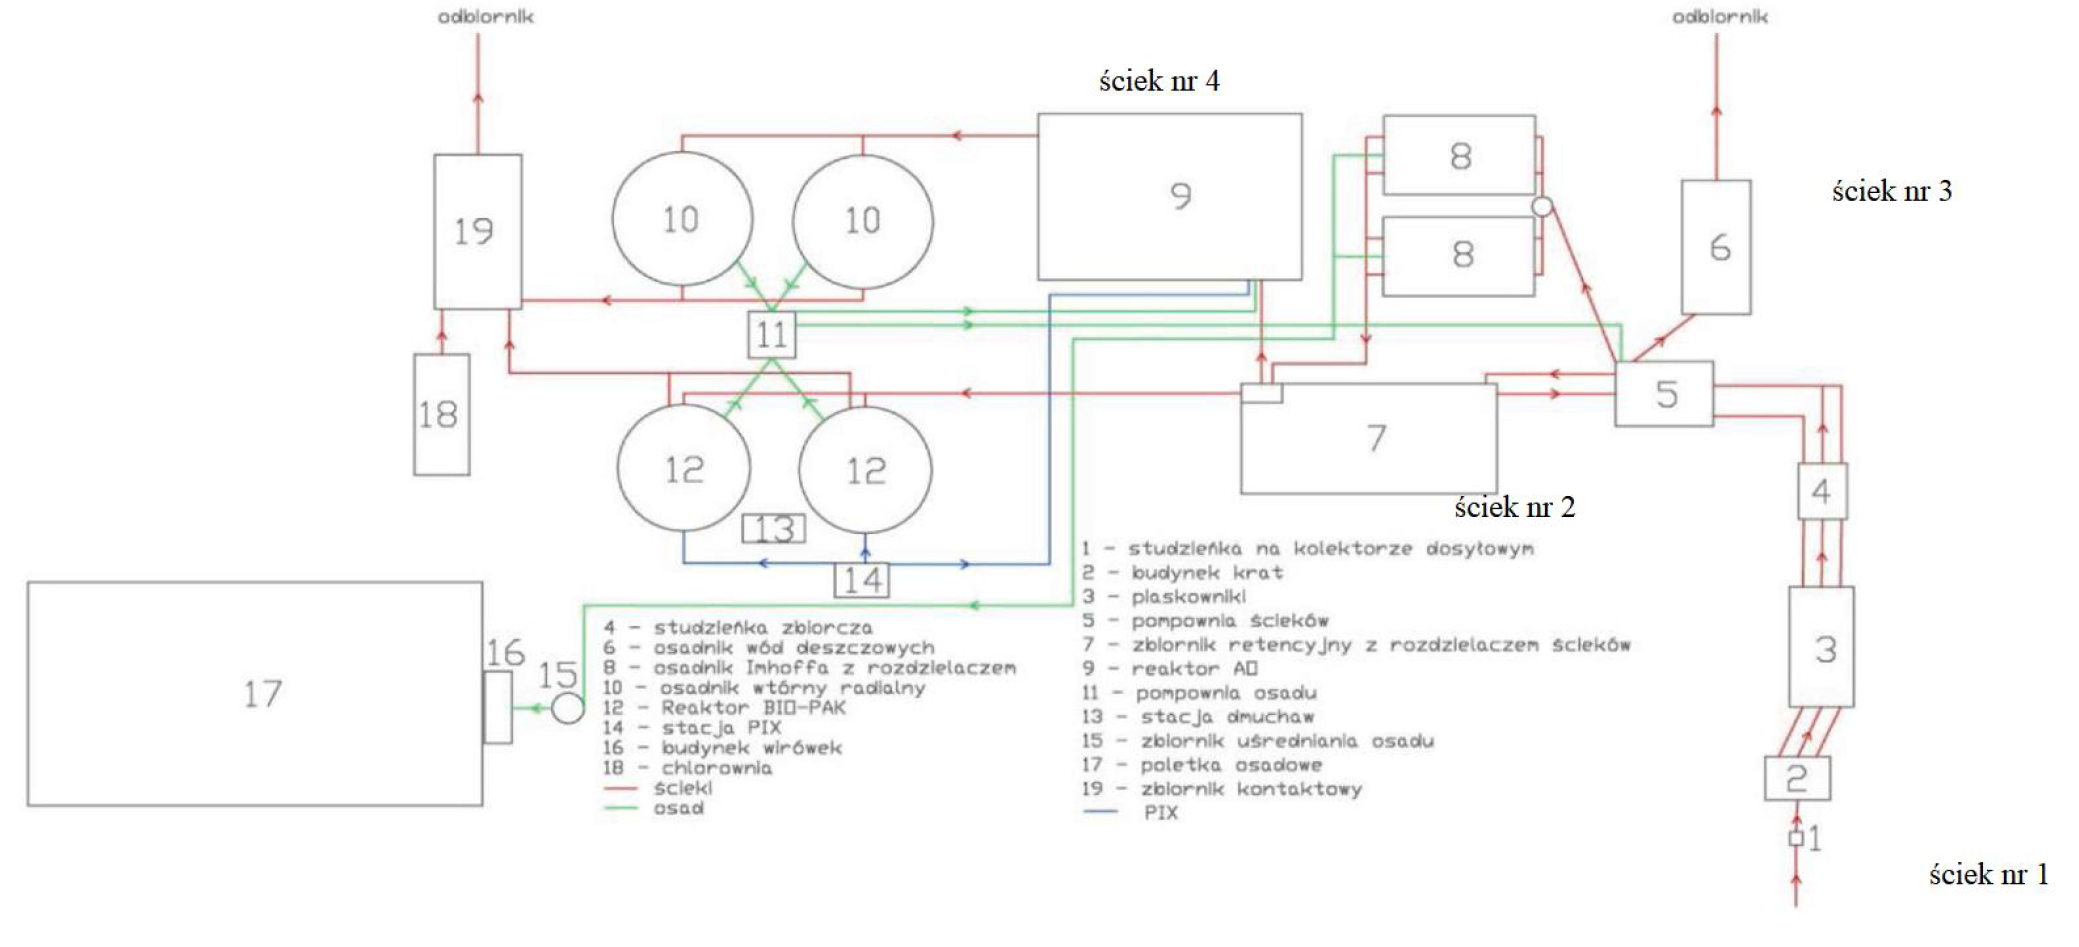
\includegraphics[width=\textwidth]{figures/wwtp}
    \caption{
        Schemat oczyszczalni ścieków w Myślenicach
        (Zaczerpnięto z: Miernik, W., Młyński, D., Chmielowski, K.,
        \& amp; Karwacki, P. (1AD). WPŁYW ŚCIEKÓW
        OCZYSZCZONYCH NA OCZYSZCZALNI W MYŚLENICACH NA JAKOŚĆ WÓD ICH ODBIORNIKA.
        INFRASTRUKTURA I EKOLOGIA TERENÓW WIEJSKICH, I(1), 191–207.)
        Na rysunku oznaczono numerami 1-4 etapy oczyszczania, na których
        zostały pobrane badane później \acrshort{ww}.}
\end{figure}

\vspace{1cm}

\begin{table}[h!]
    \label{tab:1}
    \centering
    \caption{
        Opis próbek \acrshort{ww}1-4, które zostały pobrane
        z oczyszczalni ścieków w Myślenicach (rys.~\ref{fig:5}).
    }
    \begin{tabular}{rp{10cm}}
        Numer \acrshort{ww} & Opis\\
        \hline
        1 & Ścieki surowe, zawierające również odpady stałe\\
        2 & Ścieki po usunięciu lipidów (flotacji)\\
        3 & Ścieki po kontakcie z osadem czynnym \newline (procesy beztlenowe, stary zbiornik)\\
        4 & Ścieki po kontakcie z osadem czynnym \newline (naprzemiennie procesy tlenowe i beztlenowe, cykl ok.\ 3~h)\\
    \end{tabular}
\end{table}

\vspace{\fill}

\newpage
\thispagestyle{empty}

\begin{figure}
    \centering
    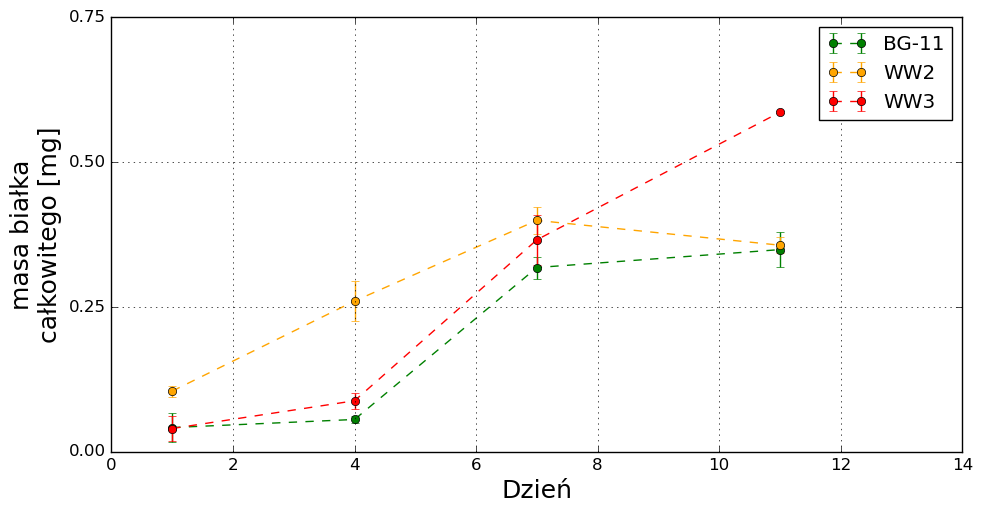
\includegraphics[width=12.5cm]{figures/totalprot}
    \caption{
        Zależność zawartości białka całkowitego od czasu w próbkach
        z eksperymentu~\ref{subsec:mlra}. Wartości były początkowo
        mierzone w celu normalizacji wyników aktywności \acrshort{mlra}.
    }
    \label{fig:6}
\end{figure}

\begin{figure}
    \label{fig:7}
    \centering
    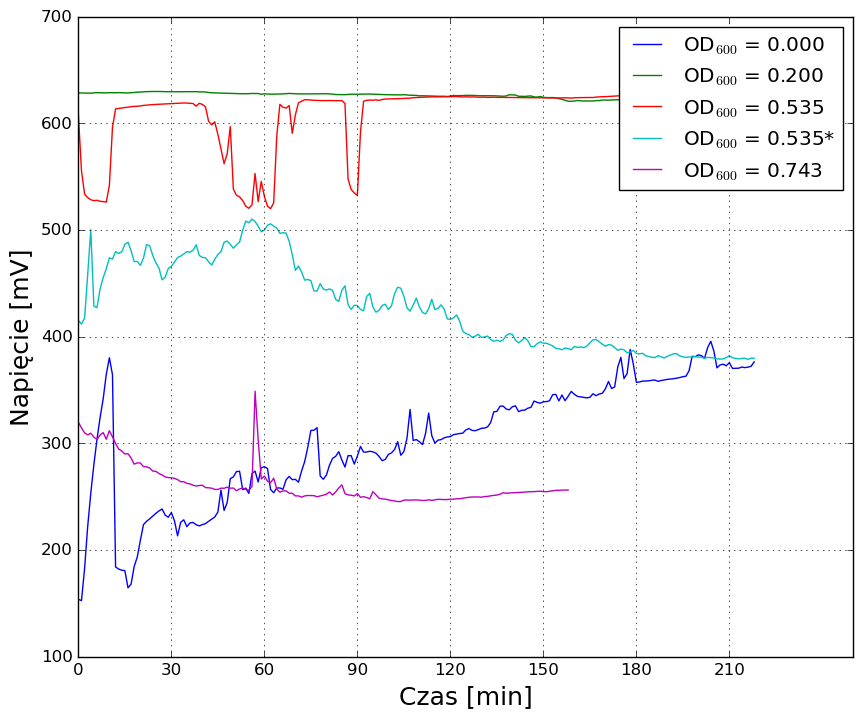
\includegraphics[width=12.5cm]{figures/voltage1}
    \caption{
        Wykres pomiarów napięcia w układzie \acrshort{amfc}
        w czasie w zależności od gęstości hodowli
        \textit{R. sphaeroides} umieszczonej w komorze z anodą.
        * Oznacza pomiar po 24~h adaptacji mikroorganizmów
        do anody.
    }
\end{figure}
